\documentclass[12pt,xcolor=usenames,dvipsnames]{beamer}
\usetheme{CambridgeUS}

\usepackage[utf8]{inputenc}
\usepackage[T1]{fontenc}
\usepackage[czech]{babel}
\usepackage{lmodern}
\usepackage{amsmath}
\usepackage{amsfonts}
\usepackage{amssymb}
\usepackage{graphicx}
\usepackage{fancyvrb} %Verbatim 

\usefonttheme{serif}

\author[Jan Šlahora]{Jan Šlahora, Jaroslav Marek}
\title{Obhajoba diplomové práce}
\subtitle{Matematická lingvistika a překlady básně E.A. Poea Havran}
%\logo{}
\institute[FEI UPCE]{Fakulta elektrotechniky a informatiky\\Univerzita Pardubice} % (optional)
%\date{}
%	\subject{}
%\setbeamercovered{transparent}
%\setbeamertemplate{navigation symbols}{}


\setlength{\parindent}{0em}
\setlength{\parskip}{1em}

\begin{document}

\frame{\titlepage}

\begin{frame}
	\frametitle{Cíle diplomové práce}

	Práce se zabývá studiem vybraných modelů matematické lingvistiky.
	
	Studované modely jsou následně aplikovány na české překlady básně Havran Edgara Allana Poea.

	K tomu je použita aplikace, jež byla v rámci diplomové práce pro tyto potřeby vytvořena.
\end{frame}

\begin{frame}
	\frametitle{Studované jevy}

	V rámci diplomové práce byly studovány jevy:
	
	\begin{itemize}
		\item frekvenční,
		\item fonické,
		\item sémiotické.
	\end{itemize}
\end{frame}

\begin{frame}
	\frametitle{Studované jevy: frekvence znaků}
	
	\vspace{-8.8pt}
	\begin{center}
		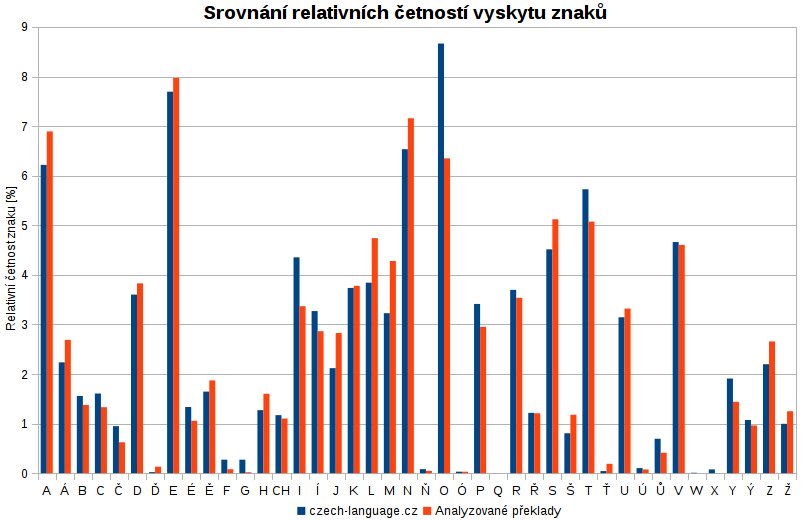
\includegraphics[width=\linewidth,height=0.86\textheight,keepaspectratio]{cetnost-znaku}
	\end{center}

\end{frame}

\begin{frame}
	\frametitle{Studované jevy: frekvence slov}
	\framesubtitle{Frekvenční slovník českých překladů}

	\vspace{-8.8pt}
	\begin{center}
		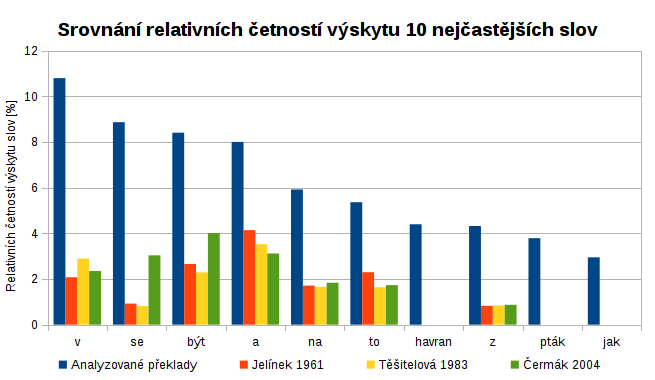
\includegraphics[width=\linewidth,height=0.86\textheight,keepaspectratio]{cetnost-slov}
	\end{center}

\end{frame}

\begin{frame}
	\frametitle{Studované jevy: frekvence slov}
	\framesubtitle{Srovnání frekvencí originálu s překlady}

	\begin{center}
		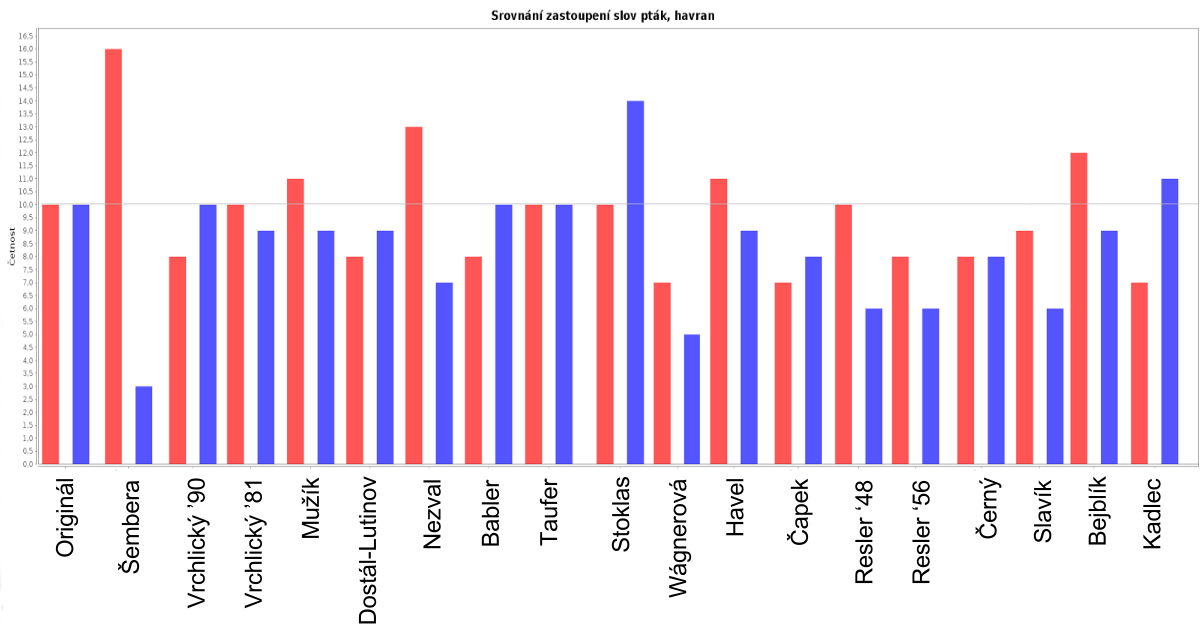
\includegraphics[width=\linewidth,height=0.86\textheight,keepaspectratio]{cetnost-slov-orig}
	\end{center}

\end{frame}

\begin{frame}
	\frametitle{Studované jevy: denotační analýza}

	Principem denotační analýzy je rozložení textu na jednotky (slova, fráze, …) a rozdělení těchto jednotek do skupin zvaných hřeby.

	Hřeb sdružuje jednotky vztahující se k jednomu a tomu samému subjektu.

	Denotační analýza zkoumá, jak spolu jednotlivé hřeby souvisí z~	hlediska morfologie, syntaxe a sémantiky.

\end{frame}

\begin{frame}[fragile]
	\frametitle{Studované jevy: denotační analýza}
	\framesubtitle{Příprava textu}

	\vspace{-10pt}
	\begin{footnotesize}
		\begin{Verbatim}[commandchars=+\[\]]
			 1|2   3   4    5       6      7|8       9    10
			Bylo pusto o půlnoci, když +underline[jsem hloubal] bez pomoci,
			
			 11|12   13    14   15   16     17     18
			luštil marně živou mocí staré svazky kajícné,
			
			    19|20      21|22    23  24   25  26  27   28
			+underline[nedřímal jsem], nebděl  ani, když tu ťuk ťuk znenadání
			
			  29|30      31         32     33  34  35
			+underline[ozvalo se] zaklepání, zaklepání a  víc  ne.
			
			 36  37  38|39  40 41|42  43     44       45
			„Kdo mě  shání, co chce  toto zaklepání kajícné?
			
			46|47  48  49  50  51  52 53
			Je     to host a  nic víc ne.“
		\end{Verbatim}	
	\end{footnotesize}

\end{frame}

\begin{frame}
	\frametitle{Studované jevy: denotační analýza}
	\framesubtitle{Etablované hřeby}

	\vspace{-15pt}
	\begin{footnotesize}
		\begin {table}[H]
		\begin{center}
			\begin{tabular}{|p{10cm}|c|c|}
				\hline 
				\bfseries Hřeb & \bfseries R & \bfseries P \\ \hline
				\textbf{6 já} [(hloub)al jsem 8, (lušti)l 12, (nedříma)l jsem 20, (nebdě)l 22, mě 37], \textbf{25 zaklepání} [(ozva)lo se 30, zaklepání 31, zaklepání 32, (chc)e 42, zaklepání 44] 
				& 5 & 2 \\ \hline
				
				\textbf{1 pusto} [(byl)o 2, pusto 3], \textbf{2 být} [bylo 1, je 46], \textbf{5 když} [když 6, když 24], \textbf{27 a} [a 33, a 50], \textbf{28 víc} [víc 34, víc 52], \textbf{29 ne} [ne 35, ne 53], \textbf{30 kdo} [kdo 36, (shán)í 39], \textbf{18 kajícný} [kajícné 18, kajícné 45], \textbf{23 ťuk} [ťuk 26, ťuk 27], \textbf{34 to} [toto 43, to 48], \textbf{35 host} [(je) 47, host 49] 
				& 2 & 11\\ \hline
				
				\textbf{3 o} [o 4], \textbf{4 půlnoc} [půlnoci 5], \textbf{7 hloubat} [hloubal jsem 7], \textbf{8 bez} [bez 9], \textbf{9 pomoc} [pomoci 10], \textbf{10 luštit} [luštil 11], \textbf{11 marně} [marně 13], \textbf{14 živou} [živou 14], \textbf{15 moc} [mocí 15], \textbf{16 starý} [staré 16], \textbf{17 svazek} [svazky 17], \textbf{19 dřímat} [nedřímal jsem 19], \textbf{20 bdít} [nebděl 21], \textbf{21 ani} [ani 23], \textbf{22 tu} [tu 25], \textbf{24 znenadání} [znenadání 28], \textbf{26 ozývat} [ozvalo se 29], \textbf{31 shánět} [shání 38], \textbf{32 co} [co 40], \textbf{33 chtít} [chce 41], \textbf{36 nic} [nic 51]
				& 1 & 21 \\ \hline
		
			\end{tabular} 
		\end{center}
	\end{table}
	\end{footnotesize}
\end{frame}

\begin{frame}
	\frametitle{Studované jevy:  denotační analýza}
	\framesubtitle{Koincidence}

	Koincidence je definována jako výskyt dvou hřebů v jednom verši. Existují koincidence:
	
	\begin{description}
		\item[náhodné] pokud pravděpodobnost výskytu daných dvou hřebů je dostatečně vysoká,
		\item[signifikantní] v případě, že pravděpodobnost tohoto výskytu je malá.
	\end{description}

	Hranice mezi náhodnou a signifikantní koincidencí je označena $\alpha$.	

\end{frame}

\begin{frame}
	\frametitle{Studované jevy:  denotační analýza}
	\framesubtitle{$\alpha$-graf}

	\vspace{-15pt}
	\begin{equation*}
		P(X \geq x)=\sum_{i=x}^{min{\left(  M, n \right) }} \frac{\binom{M}{i}\binom{N-M}{n-i}}{\binom{N}{n}},
	\end{equation*}
	\vspace{-16pt}
	\begin{small}
		kde
		\vspace{5pt} 
		\begin{align*}
			N & \text{ je počet vymezených částí textu (počet veršů, vět, slok, \ldots),}\\
			M & \text{ je počet vymezených částí, v nichž se vyskytuje hřeb $A$,}\\
			n & \text{ je počet vymezených částí, v nichž se vyskytuje hřeb $B$,}\\
			x & \text{ je počet vymezených částí, v nichž se vyskytují oba hřeby.}
		\end{align*}  
	\end{small}

	\vspace{-35pt}
	Z vypočítaných pravděpodobností $P(X\geq x)$ je možné sestrojit $\alpha$-graf. V $\alpha$-grafu jsou hřeby zakresleny jako vrcholy, přičemž sousedními se stanou ty vrcholy (=hřeby), jejichž vzájemná pravděpodobnost $P(X\geq x)$ je menší nebo rovna $\alpha$ (tzn., jsou signifikantní ).

\end{frame}

\begin{frame}
	\frametitle{Studované jevy:  denotační analýza}
	\framesubtitle{Přehled indexů nespojitosti, neizolovanosti a dosažitelnosti}

	\begin{tabular}{| p{4.1cm}|p{7.0cm}|}
	\hline
		\bfseries 
		\mbox{Indexy nespojitosti/} neizolovanosti/ \mbox{dosažitelnosti} & \bfseries Překlady \\ 
	\hline $0{,}018$/$0{,}273$/---       & A. E. Mužík, D. Wagnerová \\ 
	\hline $0{,}067$/$0{,}333$/$0{,}5$	 & V. K. Šembera, A. Bejblík \\ 
	\hline $0{,}067$/$0{,}333$/---       & E. Stoklas, K. Resler 1948 \\ 
	\hline $0{,}067$/$0{,}400$/---       & \textbf{E. A. Poe}, K. Dostál-Lutinov, R. Havel, R. Černý, I. Slavík \\ 
	\hline $0{,}067$/$0{,}500$/---       & V. Nezval, O. F. Babler, J. B. Čapek \\ 
	\hline 
	\end{tabular} 
	
	\vspace{-5pt}
	Pět překladů je charakterizováno unikátními indexy: překlad Kamila Reslera vydaný roku 1948, překlady Jaroslava Vrchlického z let 1881 a 1890, překlad Svatoupluka Kadlece a překlad Jiřího Taufera.

\end{frame}

\begin{frame}
	\frametitle{Odpovědi na připomínky práce}

	\begin{enumerate}
		\item Proč jste vybral pro analýzu 14. strofu?
		\item Jak se liší grafy, pokud hřeby vytváří různé osoby?
		\item Vysvětlete na některém překladu aliteraci, agregaci a asonanci.				
		\item Jak složitá byla algoritmizace studované problematiky?				
	\end{enumerate}
\end{frame}

\begin{frame}
	\frametitle{Odpovědi na připomínky práce}
	\framesubtitle{Proč jste vybral pro analýzu 14. strofu?}

	Po konzultaci s vedoucím DP jsme přistoupili k omezení analyzovaných básní na pouze jednu strofu.
	
	Grafy vytvořené na základě denotační analýzy čtrnácté strofy byly „zajímavější“ (obsahovaly více komponent a hran) než grafy vytvořené na základě jiných strof.
\end{frame}

\begin{frame}
	\frametitle{Odpovědi na připomínky práce}
	\framesubtitle{Jak se liší grafy, pokud hřeby vytváří různé osoby?}

	Dva možné problémy:
	
	\begin{itemize}
		\item Rozdílná pravidla pro tvorbu hřebů (resp. jejich rozdílná aplikace).
		\item Rozdílné pochopení analyzovaného textu.
	\end{itemize}
\end{frame}

\begin{frame}
	\frametitle{Odpovědi na připomínky práce}
	\framesubtitle{Vysvětlete na některém překladu \textbf{agregaci}, aliteraci a asonanci.}
	\begin{center}
	
		\textsc{Edgar Allan Poe -- Havran} {\tiny (překlad E. A. Mužík)}
	
		\emph{V půlnoc jednu pustou, tmavou,\\
		když jsem se skloněnou hlavou\dots}

		\begin{tiny}
			\begin{align*}
				A_1 &= \text{\{ \textbf{A} C \textbf{D} \textbf{E}       \textbf{J}     \textbf{L}   \textbf{M} \textbf{N} \textbf{N} \textbf{O} \textbf{O} \textbf{O} P P \textbf{S} T T \textbf{U} \textbf{U} U U U Ů \textbf{V} V \}}\\
				A_2 &= \text{\{ \textbf{A}   \textbf{D} \textbf{E} E Ě H \textbf{J} K K \textbf{L} L \textbf{M} \textbf{N} \textbf{N} \textbf{O} \textbf{O} \textbf{O}     \textbf{S} S S \textbf{U} \textbf{U} \textbf{V} Y Ž \}}\\
				B_1 &= \text{\{ \textbf{AV} CJ DN ED JE LN MA                   \textbf{NO} NU OC \textbf{OU} \textbf{OU} PU PŮ ST TM TO UP US UT ŮL \textbf{VO} VP \}}\\   
				B_2 &= \text{\{ \textbf{AV} DY EM ES ĚN HL JS KD KL LA LO MS NĚ \textbf{NO} ON    \textbf{OU} \textbf{OU} SE SE SK UH \textbf{VO} YŽ ŽJ \}}
			\end{align*}
		\end{tiny}
	
		\vspace{-50pt}
		\begin{footnotesize}
		\begin{equation*}
			S_{1,2}=100 \times \left ( \frac{\left | A_i \bigcap A_j \right |^{2}}{\left | A_i \right | \times \left | A_j \right |} + \frac{\left | B_i \bigcap B_j \right |^{2}}{\left | B_i \right | \times \left | B_j \right |} \right ) = 100 \times \left ( \frac{15^{2}}{24 \times 25} + \frac{5^{2}}{23 \times 24} \right ) \approx  42,03
		\end{equation*}
		
	\end{footnotesize}

	\end{center}


\end{frame}

\begin{frame}
	\frametitle{Odpovědi na připomínky práce}
	\framesubtitle{Vysvětlete na některém překladu \textbf{agregaci}, aliteraci a asonanci.}
	\vspace{-8pt}
	\begin{center}
		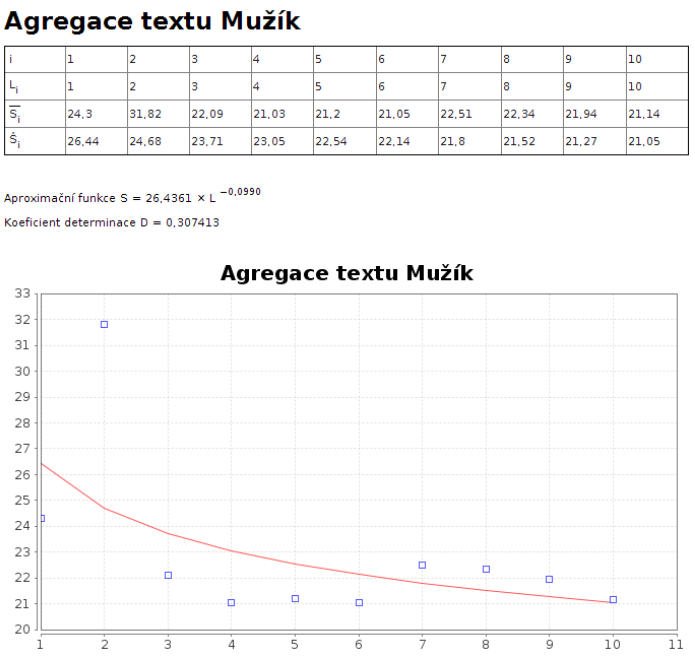
\includegraphics[width=\linewidth,height=0.8\textheight,keepaspectratio]{agregace}
	\end{center}

\end{frame}

\begin{frame}
	\frametitle{Odpovědi na připomínky práce}
	\framesubtitle{Vysvětlete na některém překladu agregaci, \textbf{aliteraci} a asonanci.}

	\begin{center}
	
		\textsc{Edgar Allan Poe -- Havran} {\tiny (překlad Jaroslav Vrchlický 1881)}
	
		\emph{\textbf{\textcolor{blue}{H}}edvábná \textbf{\textcolor{Red}{s}}e \textbf{\textcolor{blue}{h}}nula \textbf{\textcolor{Green}{c}}lona, \textbf{\textcolor{Green}{c}}os \textbf{\textcolor{Orchid}{v}} \textbf{\textcolor{BurntOrange}{n}}í šustí, \textbf{\textcolor{Green}{c}}os \textbf{\textcolor{Orchid}{v}} \textbf{\textcolor{BurntOrange}{n}}í \textbf{\textcolor{Red}{s}}toná,\\
mysl plní se a vlní, bázně také neznajíc,\\
takže srdce si dodávám, vstávám a si předříkávám:\\
„Chodec to, ždá nocleh sobě, bloudě kol mých okenic,\\
nějaký to chodec pozdní bloudí u mých okenic --\\
        to je to a pranic víc.“\\\dots}

	\end{center}
\end{frame}


\begin{frame}
	\frametitle{Odpovědi na připomínky práce}
	\framesubtitle{Vysvětlete na některém překladu agregaci, \textbf{aliteraci} a asonanci.}

	\begin{equation*}
		{K\!A}_{E.A.Poe} = 3{,}79759
	\end{equation*}
{\footnotesize 
	\begin{tabular}{|lr|lr|lr|}
\hline \bfseries Text & \bfseries $KA_{\text{báseň}}$ & \bfseries Text & \bfseries $KA_{\text{báseň}}$ & \bfseries Text & \bfseries $KA_{\text{báseň}}$ \\ 
\hline Mužík          & 1,58133                       & Resler ‘56     & 3,33302                       & Šembera        & 3,57143 \\ 
\hline Vrchlický ‘90  & 1,76623                       & Taufer         & 3,36161                       & Dostál-Lutinov & 3,58246 \\ 
\hline Wagnerová      & 1,98075                       & Resler ‘48     & 3,48301                       & Vrchlický ‘81  & 3,64690 \\ 
\hline Čapek          & 3,09970                       & Babler         & 3,49542                       & Kadlec         & 3,66010 \\ 
\hline Nezval         & 3,14763                       & Slavík         & 3,53020                       & Stoklas        & 3,87856 \\ 
\hline Havel          & 3,28966                       & Černý          & 3,56506                       & Bejblík        & 3,99667 \\ 
\hline 
\end{tabular} 
}

\end{frame}

\defverbatim{\ason0}{%
\begin{footnotesize}
\begin{Verbatim}[commandchars=\\\{\},codes={\catcode`$=3\catcode`^=7\catcode`_=8}]


\end{Verbatim}
\end{footnotesize}
}

\defverbatim{\asonA}{%
\begin{footnotesize}
\begin{Verbatim}[commandchars=\\\{\},codes={\catcode`$=3\catcode`^=7\catcode`_=8}]
O, E, U, O, A, I, I, E, A, Y, I, E, I, O, E, E, E, A, A, E, A, Y

\end{Verbatim}
\end{footnotesize}
}

\defverbatim[colored]{\asonB}{%
\begin{footnotesize}
\begin{Verbatim}[commandchars=\\\{\},codes={\catcode`$=3\catcode`^=7\catcode`_=8}]
\textcolor{gray}{O}, E, U, O, A, I, \textcolor{red}{I}, E, A, Y, \textcolor{red}{I}, E, I, O, E, \textcolor{red}{E}, \textcolor{red}{E}, A, \textcolor{red}{A}, E, A, Y
   O, E, U, O, A, \textcolor{red}{I}, I, E, A, \textcolor{red}{Y}, I, E, I, O, \textcolor{red}{E}, \textcolor{red}{E}, E, \textcolor{red}{A}, A, E, A, \textcolor{gray}{Y}
\end{Verbatim}
\end{footnotesize}
}

\begin{frame}[fragile]
	\frametitle{Odpovědi na připomínky práce}
	\framesubtitle{Vysvětlete na některém překladu agregaci, aliteraci a \textbf{asonanci}.}

	\only<1->
	{
		\begin{center}
			\textsc{Edgar Allan Poe --- The Raven}
		
			{\small \emph{Once upon a midnight dreary, while I pondered, weak and weary,\\
		Over many a quaint and curious volume of forgotten lore --\\
		While I nodded, nearly napping, suddenly there came a tapping\ldots}}
	
		\end{center}
	}
\only<1>{
\ason0
}	
\pause

\only<2>{
\asonA
}


\only<3>{
\asonB
}


\end{frame}	

\begin{frame}[fragile]
	\frametitle{Odpovědi na připomínky práce}
	\framesubtitle{Vysvětlete na některém překladu agregaci, aliteraci a \textbf{asonanci}.}

	V rámci DP byla provedena analýza zkoumající, zda se liší hodnoty asonance pro různé posuny. 
	
	Testovány byly posuny o 1 až 15 vokálů. 
	
	Analýza odhalila, že se hodnoty asonance pro různé posuny liší:

	{\small \begin{tabular}{|l|l|l|l|}
		\hline Posun o 1 a 7  & Posun o 3 a 7 & Posun o 5 a 14 & Posun o 8 a 11  \\ 
		\hline Posun o 1 a 8  & Posun o 3 a 8 & Posun o 7 a 11 & Posun o 8 a 12  \\ 
		\hline Posun o 1 a 14 & Posun o 5 a 7 & Posun o 8 a 9  & Posun o 8 a 13  \\ 
		\hline Posun o 2 a 8  & Posun o 5 a 8 & Posun o 8 a 10 & Posun o 11 a 14 \\ 
		\hline 
	\end{tabular} }


\end{frame}

\begin{frame}
	\frametitle{Odpovědi na připomínky práce}
	\framesubtitle{Jak složitá byla algoritmizace studované problematiky?}

	Složitost se pohybovala od lehké (výpočet frekvence znaků a slov) přes složitější (fonické jevy) po velmi komplexní (denotační analýza).

	Ta sestává ze dvou částí: dělení textu do hřebů a zobrazení výsledků analýzy.

	Implementace dělení textu do hřebů byl z hlediska vývoje nejnáročnější úkol  z celé DP.

\end{frame}

\begin{frame}
\begin{block}{}
\begin{center}
\textcolor{Maroon}{\textbf{{\huge Děkuji za pozornost!}}}
\end{center}
\end{block}
\end{frame}

\end{document}